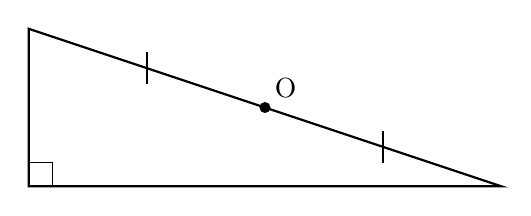
\begin{tikzpicture}[scale=1]

    % --- Coordinates ---
    % Defining points for the right-angled triangle based on Figure 18
    \coordinate (V) at (0,2);   % Top-left vertex
    \coordinate (B) at (0,0);   % Bottom-left vertex (Right Angle)
    \coordinate (C) at (6,0);   % Bottom-right vertex
    \coordinate (O) at (3,1);   % Midpoint O on the hypotenuse VC

    % --- Lines ---
    % Draw the main triangle sides
    \draw[thick] (V) -- (B) -- (C) -- cycle;

    % --- Right Angle Symbol ---
    % Square symbol at vertex B as shown in Figure 18
    \draw (0,0.3) -- (0.3,0.3) -- (0.3,0);

    % --- Midpoint Marker ---
    % Draw the point dot for O on the hypotenuse
    \fill (O) circle (2pt);

    % --- Equality Tick Marks ---
    % Ticks on the hypotenuse to show the segments are equal (VO = OC)
    
    % Tick on segment VO
    \draw[thick] (1.5, 1.7) -- (1.5, 1.3);
    
    % Tick on segment OC
    \draw[thick] (4.5, 0.7) -- (4.5, 0.3);

    % --- Labels ---
    % Positioning the label 'O' above the point as seen in Figure 18
    \node[above right] at (O) {O};

\end{tikzpicture}